\RequirePackage{amsmath}
\documentclass[runningheads]{llncs}

\usepackage{textcomp}
\usepackage{framed}
\let\proof\relax
\let\endproof\relax
\usepackage{amsthm}
\usepackage{mathtools}
\usepackage{hyperref}
\usepackage{fnpct}
\usepackage{enumitem}
\usepackage{dirtree}
\usepackage{listings}
\lstset{
language=Java,
columns=flexible,
numbers=left,
xleftmargin=3em,
frame=single,
framexleftmargin=3em,
keywordstyle=\rmfamily,
moredelim=[s][\rmfamily]{/*@}{*/},
moredelim=[l][\rmfamily]{//@}}

% Use multiple bibliographies
\usepackage{multibib}
\newcites{Self}{Self-references}

\makeatletter
\DeclareRobustCommand*{\lyxarrow}{%
\@ifstar
{\leavevmode\,$\triangleleft$\,\allowbreak}
{\leavevmode\,$\triangleright$\,\allowbreak}}
\makeatother

\def\bs{\char092}

\begin{document}
% This makes sure lstlisting counts without section number, just like figures
\renewcommand{\thelstlisting}{\arabic{lstlisting}}

\title{A Tutorial on Verifying \texttt{LinkedList} using KeY}
\author{{Hans-Dieter} A. Hiep\orcidID{0000-0001-9677-6644}\footnote{Corresponding author: \texttt{hdh@cwi.nl}} \and Jinting Bian \and\\
Frank S. de Boer \and Stijn de Gouw}
\authorrunning{H.A. Hiep, J. Bian, et al.}

\institute{CWI, Science Park 123, 1098 XG Amsterdam, The Netherlands\\
\email{\{hdh,j.bian,frb,stijn.de.gouw\}@cwi.nl}}

\maketitle

\begin{abstract}
This is a tutorial paper on using KeY to demonstrate formal verification of state-of-the-art, real software. In sufficient detail for a beginning user of JML and KeY, the specification and verification of part of a corrected version of the \texttt{java.util.LinkedList} class of the Java Collection framework is explained. The paper includes video material that shows recordings of interactive sessions \citeSelf{Bian2020collection}, and project files with solutions \citeSelf{10.5281/zenodo.3613712}. As such, it is also interesting for the expert user and the developer of KeY, as a `benchmark' that could lead to improvement of the specification language, user interaction, and (automatic) proof strategies.
\end{abstract}

\keywords{KeY, Java Modeling Language, cyclic data structure, case study}

\section{Introduction}

Software libraries are the building blocks of many programs that run on the devices of many more users every day. The functioning of a system may rely for a large part on its used software libraries. A small error present in a heavily-used software library could lead to serious unwanted outcomes, such as system outages and failures. Using informal root cause analysis \cite{rooney2004root}, one could find from a system failure its root causes, which may include programming errors. But root cause analysis can only applied \emph{after} a failure has happened. To prevent certain failures from happening in the first place, program correctness is of the utmost importance. Although establishing program correctness seems to be an expensive activity, it may be worthwhile for critical software libraries, such the standard library that all programs rely on.

This tutorial intends to show how we take an existing Java program that is part of the Java standard library, and study it closely to increase our understanding of it. If we are only interested in showing the presence of an issue with the program, e.g.~that it lacks certain functionality, it suffices to show an example run which behaves unexpectedly. But to reach the conclusion that no unexpected behavior ever results from running the program, first requires a precise specification of what behavior one expects, and further requires a convincing argument that all possible executions of the program exhibit that behavior.

We take a formal approach to both specification and reasoning about program executions, allowing us to increase the reliability of our reached conclusions. In particular, the specifications we write are expressed in the Java Modeling Language (JML), and our reasoning is tool-supported and partially automated by KeY. To the best of the authors' knowledge, KeY is the only tool that supports enough features of the Java programming language for reasoning about real programs, of which its run-time behavior crucially depends on the presence of features such as: dynamic object creation, exception handling, integer arithmetic with overflow, \texttt{for} and \texttt{foreach} loops with early returns, nested classes (both static and non-static), inheritance, polymorphism, erased generics, etc.

As a demonstration of applying KeY to state-of-the-art, real software, we will focus on Java's \texttt{LinkedList} class, for two reasons. First, a (doubly-)linked list is a well-known basic data structure for storing and maintaining unbounded data, and has many applications: for example, in Java's secure sockets implementation. Second, it has turned out that there is a 20-year-old bug lurking in its program, that might lead to security-in-depth issues on large memory systems, caused by the overflow of a field that caches the length of the list \citeSelf{hiep2019verifying}. Our specification and verification effort will be aimed at establishing the absence of this bug from a repaired program.

This article is based on the results as described in another closely related paper \citeSelf{hiep2019verifying}. That paper provides a high-level overview on the specification and verification effort of the linked list class as a whole, for a more general audience. In the present article, more technical details how we use the KeY theorem prover are given, and we give more detail concerning the production of the proofs. In particular, this tutorial consists of the on-line repository of proof files \citeSelf{10.5281/zenodo.3613712}, and on-line video material that shows how to (re)produce the proofs \citeSelf{Bian2020addbranch,Bian2020lemma}: these are video recordings of the interactive sessions in KeY that demonstrates exactly what steps one could take to complete the correctness proofs of the proof obligations generated by KeY from the method contracts.

\paragraph{Contents}
We see how to set-up a project and configure the KeY tool (Section~\ref{sec:setup}).
We then study the source code of the \texttt{LinkedList} to gain intuitive understanding of its structure:
how the instances look like, and how the methods operate (Section~\ref{sec:linkedlist}).
%A basic introduction to the KeY system is given, on which the rest of the tutorial is based (Section~\ref{sec:background}).
We formulate, based on previous intuition, a \emph{class invariant} in JML that expresses a property that is true of every instance (Section~\ref{sec:class-invariant}).
An interesting property that follows from the class invariant, that is used as a separation principle, is described next (Section~\ref{sec:acyclicity}).
To keep this presentation reasonably short, we further focus on the methods which pose the main challenges to formal verification, \texttt{add} and \texttt{remove}. We give a \emph{method contract} for the \texttt{add} method that describes its expected behavior and we verify that its implementation is correct (Section~\ref{sec:add}). The difficulty level increases after we specify the \texttt{remove} method (Section~\ref{sec:remove}), as its verification requires more work than before. We study a deeper method that \texttt{remove} depends on, and finally use \emph{loop invariants} to prove the correctness of \texttt{remove}.
We conclude with some methods of \texttt{LinkedList} left as exercise to the reader (Section~\ref{sec:conclusion}): finding their specifications and proving them correct is not trivial, but done in a similar way.

\section{Set-up}\label{sec:setup}

\begin{table}
\dirtree{%
.1 linkedlist-tutorial.
.2 key-2.6.3.zip.
.2 LinkedList.key.
.2 src.
.3 java.
.4 util.
.5 LinkedList.java.
.5 LinkedList.solution.
.2 jre.
.3 java.
.4 ....
.2 proof.
.3 ....
}
\medskip
    \caption{Directory structure of project files. The \texttt{src} directory contains the Java classes we want to specify and verify. The \texttt{jre} directory contains stub files, with specifications of unrelated classes. The \texttt{LinkedList.solution} file is the source file we end up with after following this tutorial. The \texttt{proof} directory contains the completed proofs.}
    \vspace*{-20pt}
    \label{tab:directory-structure}
\end{table}

First we will set-up the project files needed to use KeY. The project files are available on-line \citeSelf{10.5281/zenodo.3613712}: these can be downloaded and include the KeY software version that we use. After unpacking the project files, we end up with the directory structure of Table~\ref{tab:directory-structure}.

The original source file of \texttt{LinkedList.java} was obtained from OpenJDK version \texttt{jdk8-b132}. The original has been pre-processed: generic class parameters are removed, and all methods and nested classes irrelevant to this tutorial are removed. Both the removal of generics and the stub files in the \texttt{jre} folder were generated automatically, using the Eclipse extensions for KeY. Repeating those steps is not necessary here.

Over the course of next sections, we will modify the source file and add annotations to formally specify its behavior, and helper methods for presenting intermediary lemmas. The annotations are usual Java comments, and thus ignored when the file is read by a Java compiler. The helper methods introduce slight performance overhead (of calling a method that performs no operations, and immediately returning from it); it is clear that these do not change the original behavior of the program.

\subsection{KeY settings}

\begin{table}
    \begin{tabular}{l@{\hskip6pt}|@{\hskip6pt}l}
    Max. rule applications & 1000 \\
    Stop at & Default \\
    Proof splitting & Delayed \\
    Loop treatment & Invariant \\
    Block treatment & Contract \\
    Method treatment & Contract \\
    Dependency contract & On \\
    Query treatment & Off \\
    Expand local queries & On \\
    Arithmetic treatment & Basic \\
    Quantifier treatment & No splits with progs. \\
    \textbf{Class axiom rule} & \textbf{Off} \\
    Auto induction & Off \\
    User-defined taclets & All off
    \end{tabular}
    \medskip
    \caption{The proof search strategy settings we use.}
    \vspace*{-20pt}
    \label{tab:proof-strategy}
\end{table}

To produce proofs in KeY, the first step is to set-up KeY's taclet base to make use of particular groups of rules that correctly model Java's integer overflow semantics. This has to be done only once, as these taclet settings are stored per computer user.

Sometimes, KeY overwrites or corrupts these settings if different versions are used. To ensure KeY starts in a fresh state, one can remove the \texttt{.key} directory from the user's home directory, and clean out preferences from the \texttt{.java/.userPrefs} directory by deleting the \texttt{de/uka/ilkd/key} hierarchy containing \texttt{prefs.xml} files\footnote{On Windows, the preferences are instead stored in the Windows Registry. Use the \texttt{regedit} tool and clean out under \texttt{HKEY\_CURRENT\_USER\bs Software\bs JavaSoft\bs Prefs} or \texttt{HKEY\_CURRENT\_USER\bs Software\bs Wow6432Node\bs JavaSoft\bs Prefs} the same hierarchy. On Mac OS, open a terminal, change directory to \texttt{\textasciitilde/Library/Preferences} and delete \texttt{de.uka.ilkd.plist}}.

Now start up KeY, and the example selection screen appears (if not, selecting File\lyxarrow Load Example opens the same screen). Load any example, to enter proof mode. 
First, we set-up a proof strategy. On the right side of the window, change the settings in the Proof Search Strategy tab to match those of Table~\ref{tab:proof-strategy}. Then, select Options\lyxarrow Taclet Options, and configure the options as in Table~\ref{tab:taclet-options}.

The taclet options become effective after loading the next problem. We do that now: the main proof file \texttt{LinkedList.key} can be loaded, and a Proof Management window opens up, showing a class hierarchy and its methods. A method is not shown when no specifications for it are written. After giving specifications, what we will do below, more methods can be selected in this window.

\begin{table}
    \begin{tabular}{l@{\hskip6pt}|@{\hskip6pt}l}
    \textbf{JavaCard} & \textbf{Off} \\
    Strings & On \\
    Assertions & Safe \\
    BigInt & On \\
    Initialization & Disable static initialization \\
    \textbf{Int Rules} & \textbf{Java semantics} \\
    Integer Simplification Rules & Full \\
    Join Generate Is Weakening & Off \\
    Model Fields & Treat as axiom \\
    \textbf{More Sequence Rules} & \textbf{On} \\
    Permissions & Off \\
    Program Rules & Java \\
    Reach & On \\
    Runtime Exceptions & Ban \\
    Sequences & On \\
    Well-definedness Checks & Off \\
    Well-definedness Operator & L
    \end{tabular}
    \medskip
    \caption{The taclet options we use.}
    \vspace*{-20pt}
    \label{tab:taclet-options}
\end{table}

\section{\texttt{java.util.LinkedList}}\label{sec:linkedlist}

In this section we walk through part of the source code of Java's linked list: see the \texttt{LinkedList.java} file. Over the course of this tutorial, we add annotations at the appropriate places. We finally obtain the \texttt{LinkedList.solution} file.

\lstinputlisting[linerange=1-10,caption={The \texttt{LinkedList} class fields and constructor (begin of file).},captionpos=b,label={lst:linkedlist}]{figures/LinkedList.java}

Our \texttt{LinkedList} class has three attributes and a constructor (Listing~\ref{lst:linkedlist}). A \texttt{size} field, which stores a cached number of elements in the list, and two fields that store a reference to the first and last \texttt{Node}. The public constructor contains no statements: thus it initializes size to zero, and first and last to \texttt{null}.

The linked list fields are declared transient and package private. The transient flag is not relevant to our verification effort. The reason the fields are declared package private seems to prevent generating accessor methods by the Java compiler. However, in practice, the fields are treated as if they were private.

\lstinputlisting[firstnumber=65,linerange=65-77,caption={The \texttt{Node} nested class fields and constructor (end of file).},captionpos=b,label={lst:linkedlist-node}]{figures/LinkedList.java}

The \texttt{Node} class is defined as a private static nested class to represent the containers of items stored in the list (Listing~\ref{lst:linkedlist-node}). A static nested private class behaves like a top-level class, except that it is not visible outside the enclosing class. The nodes are doubly-linked, that is, each node is connected to its preceding node (through field \texttt{prev}) and succeeding node (through field \texttt{next}). These fields contain \texttt{null} in case no preceding or succeeding node exists. The data itself is contained in the \texttt{item} field of a node.

\lstinputlisting[firstnumber=39,linerange=39-43,caption={The method \texttt{add}.},captionpos=b,label={lst:linkedlist-add}]{figures/LinkedList.java}

The method \texttt{add} for adding elements to the list, takes one argument, the item to add (Listing~\ref{lst:linkedlist-add}). The informal Java documentation for \texttt{Collection} specifies it always returns \texttt{true}. The implementation immediately calls \texttt{linkLast}.

\lstinputlisting[firstnumber=45,linerange=45-63,caption={The method \texttt{remove}.},captionpos=b,label={lst:linkedlist-remove}]{figures/LinkedList.java}

The method \texttt{remove} for removing elements, also takes one argument, the item to remove (Listing~\ref{lst:linkedlist-remove}). If that item was present in the list, then its first occurrence is removed and \texttt{true} is returned; otherwise, if the item was not present, then the list is not changed and \texttt{false} is returned.

Presence of the item depends on whether the argument of the remove method is \texttt{null} or not. If the argument is \texttt{null}, then it searches for the first occurrence of a \texttt{null} item in the list. Otherwise, it uses the \texttt{equals} method, that every \texttt{Object} in Java has, to determine the equality of the argument with respect to the contents of the list. The first occurrence of an item that is considered equal by the argument is then returned. In both cases, the source code walks over the linked list, from the first node until it has reached the end. In the case that the node was found that contains the first occurrence of the argument, an internal method is called: \texttt{unlink}, and afterwards \texttt{true} is returned.

Observe that the linked list is not modified if \texttt{unlink} is not called. Although not immediately obvious, this requires that the \texttt{equals} method of every object cannot modify our current linked list, for the duration of the call to \texttt{remove}. When the \texttt{remove} method is called with an item that is not contained in the list, either loop eventually exits, and \texttt{false} is returned.

\lstinputlisting[firstnumber=11,linerange=11-18,caption={The internal method \texttt{linkLast}.},captionpos=b,label={lst:linkedlist-linkLast}]{figures/LinkedList.java}

The internal method \texttt{linkLast} changes the structure of the linked list (Listing~\ref{lst:linkedlist-linkLast}). After performing this method, a new node has been created, and the \texttt{last} field of the linked list now points to it. To maintain structural integrity, also other fields change: if the linked list were empty, the \texttt{first} field now points to the new, and only, node. If the linked list was not empty, then the new last node is also reachable via the former last node's \texttt{next} field. It is always the case that all items of a linked list are reachable through the \texttt{first} field, then following the \texttt{next} fields, and also for the opposite direction.

\lstinputlisting[firstnumber=20,linerange=20-37,caption={The internal method \texttt{unlink}.},captionpos=b,label={lst:linkedlist-unlink}]{figures/LinkedList.java}

The internal method \texttt{unlink} is among the most complex methods that alters the structure of a linked list (Listing~\ref{lst:linkedlist-unlink}). The method is used only when the linked list is not empty. Its argument is a node, necessarily one that belongs to the linked list. We first store the fields of the node in local variables: the old item, and next and previous node references.

After the method returns, the argument fields are all cleared, presumably to help the garbage collector. However, other fields also change: if the arguments is the first node, the \texttt{first} field is updated; if argument is the last node, the \texttt{last} field is updated. The predecessor or successor fields \texttt{next} and \texttt{prev} of other nodes are changed to maintain the integrity of the linked list: the successor of the unlinked node becomes the successor of its predecessor, and the predecessor of the unlinked node becomes the predecessor of its successor.

\begin{figure}
  \centering
  \includegraphics[width=\textwidth]{figures/linkedlist1.eps}
  \caption{Three example linked lists: empty, with a chain of one node, and with a chain of two nodes. Items themselves are not shown.}
  \label{fig:linkedlist}
\end{figure}

\subsection{Expected behavior}

We draw pictures of linked list instances to understand better how the structure looks like over time. In Fig.~\ref{fig:linkedlist}, we see three linked list instances. The left-most linked list is an object without any items: its \texttt{size} is zero. When we perform \texttt{add} with some item (it is not important what item), a new node is created and the first and last pointers are changed to point to the new node. Now the \texttt{prev} and \texttt{next} fields of the new node are \texttt{null}, indicating that there is no other node before and there is no other node after it. Also, the \texttt{size} field is increased by one. Adding another item further creates another node, that is linked up to the previous node properly; the \texttt{last} field is then pointed to the newly created node.
In the third instance, suppose we would perform \texttt{remove} with the first item. We would then have to unlink the node, see the code of \texttt{unlink} in Listing~\ref{lst:linkedlist-unlink}: the new value of \texttt{first} becomes the value of \texttt{next} which is the last node, and the value of \texttt{prev} of the succeeding node becomes the value of \texttt{prev} of the node that is unlinked, which is \texttt{null}. We thus end up in a similar situation as the second instance (except for the item that may be different). Removing the last item brings us back into the situation depicted by the first instance.

An important aspect of the implementation of our linked list is the cached \texttt{size} field: it represents the number of nodes that form a chain between \texttt{first} and \texttt{last}. It turns out an overflow may happen under certain conditions \citeSelf{hiep2019verifying}. Consider two facts: Java integer primitives are stored in signed 32-bit registers, and it is possible to create a chain that is larger than the maximum positive value that can be stored in such fields, $2^{31}-1$. Now, the cached size and the actual size no longer correspond. In the methods we have seen above, this seems to be no issue. But another method of the linked list may be used to demonstrate the key problem: \texttt{toArray}. The intention of \texttt{toArray} is to give back an array containing all the items of the list (see Listing~\ref{lst:linkedlist-toArray}). There are two problems: after the overflow has occurred and the \texttt{size} is negative, the \texttt{toArray} throws an unexpected \texttt{NegativeArraySizeException}. But, even worse, after adding more items that brings the size back to a positive integer, e.g. adding $2^{32}+1$ items in total, the returned array is of the wrong size and does not contain \emph{all} items of the list: without throwing an exception!

\lstinputlisting[numbers=none,caption={The method \texttt{toArray} has unexpected behavior.},captionpos=b,label={lst:linkedlist-toArray}]{figures/bug.java}

\subsection{Verification goal}

We thus revise the source code and add a method that implements an overflow check (see Listing~\ref{lst:linkedlist-fix}). The intention is that the overflow is signalled before it occurs, by throwing an exception. This ensures that the integrity of the linked list is always maintained. We modify the \texttt{add} method, and perform a call to this \texttt{checkSize()} method before invoking \texttt{linkLast}.

\lstinputlisting[numbers=none,caption={A new internal method \texttt{checkSize}.},captionpos=b,label={lst:linkedlist-fix}]{figures/fix.java}

Our aim in this tutorial is to keep the discussion abstract and general enough, without losing interesting particular details. We apply step-wise refinements to our arguments, where we start with a higher-level intuition and drill-down on technical details as they become relevant. The reader can always see the video material; but, a high-level intuition seems essential for following along.

Our specification and verification goals consists of two points:

\begin{enumerate}
    \item Specification captures the `intended' behavior of the methods with respect to its structural properties: in particular, we abstract away some properties pertaining to the contents of the linked list.
    \item Verification ensures the overflow bug no longer happens in the revised linked list: the actual number of nodes and the cached size are always the same.
\end{enumerate}

The specifications and proofs can be improved with regard to the first point, but this is left as an exericse to the reader (see Section~\ref{sec:conclusion}). The second point deserves some introduction: how can one be sure that for every linked list, the number of nodes and the value stored in the size field are the same? Can we, naively, keep track of the number of nodes and ensure that it never becomes larger than what a Java integer can represent? This is not sufficient, because the number of nodes depends on the success of a \texttt{remove} call: removing an item that is not present in the linked list should not affect its size, while removing an item that is present decreases its size by one. We refine: we could keep track of the items that are stored by the linked list. The structure to collect these items in cannot be a set of items, since we could have duplicate items in the list. A multiset of items, the contents of a linked list, seems right: the size field of the linked list must be the same as the size of its contents, and the remove method is only successful if its argument was contained before the call.

However, working with multisets is quite unnatural, as the \texttt{remove} method removes the first item in the list. That can be refined by specifying the contents as a sequence of items instead. Although this could work in principle, a major difficulty when verifying the \texttt{remove} method is to give an argument as to why the method terminates. This requires knowledge of the linking structure of the nodes. We could relate the sequence of items to iterated traversal over nodes, saying that the first item of a linked list is found in the node by traversing \texttt{first}, and the item at index $0<i<n$ is found in the node by traversing \texttt{first} and then \texttt{next} for $i-1$ times. Formalizing this seems quite difficult, and as we shall see, not even possible in first-order logic.

Hence, we end up with our last refinement: we keep track of a sequence of nodes. From this sequence, one obtains the sequence of items. We relate the sequence of nodes to the linked list instance and require certain structural properties to hold of the nodes in the sequence. The length of this sequence is the actual number of nodes, that we show to be equal to the cached size.

%\section{Background}\label{sec:background}

For formally specifying and verifying our linked list it is necessary to have basic knowledge of the system we are using: KeY. The main reference work on the KeY system is the KeY book \cite{KeYbook}. The KeY system consists of three main components: a proof system, a translator of Java programs annotated with JML into proof obligations, and an interactive tool for constructing proofs.

The logic underlying KeY is \emph{JavaDL}, a program logic that directly incorporates Java program fragments.
The program logic is a multi-modal logic: $\langle P\rangle\varphi$ expresses that executing the program fragment $P$ definitely terminates and $\varphi$ holds in the final state; and $[P]\varphi$ expresses \emph{if} the program fragment $P$ terminates, \emph{then} $\varphi$ holds in the final state. The formula $\varphi\to\langle P\rangle\psi$ expresses that if $\varphi$ holds in the initial state, then execution of $P$ terminates in a state for which $\psi$ holds.  See \cite[Chapter 3]{KeYbook}.

The program logic distinguishes \emph{program variables} from \emph{logical variables}: the value of a program variable can be changed over the course of executing a program, whereas a logical variable always has the same value. As logical variables can never be modified by a program fragment, they are used as so-called \emph{freeze variables}.

The proof system that KeY uses to establish validity of formulas is given as a sequent calculus. A sequent $\varphi_1,\ldots,\varphi_n \Rightarrow \psi_1,\ldots,\psi_m$ consists of $n$ antecendents and $m$ consequents, all formulas of JavaDL, with the usual interpretation: $\varphi_1,\ldots,\varphi_n \Rightarrow \psi_1,\ldots,\psi_m$ means that if all $\varphi_i$ on the left are true, then at least one $\psi_j$ on the right is true. Derivability of a sequent in the proof system is as usual by means of deduction rules, assembled into a proof tree. Next to the deduction rules for classical first-order logic, the proof system also consists of a large number of other rules.

Deduction rules are given by means of lightweight tactics (called taclets~\cite{beckert2004taclets}) that perform modifications on the sequent one is proving: e.g.~split branches in the proof tree, substitute variables, rewrite terms, or close a branch. There are approximately 1750 rules that implement symbolic execution for Java program fragments, and implement the theories of many sorts: integers, sequences, heaps, location sets, and others.

Of particular interest to us are rules concerning \emph{updates} and \emph{heaps}. There are rules that transform modalities with program fragments into so-called update modalities. Updates always terminate and they assign JavaDL terms to program variables. As such, updates cannot assign program variables to side-effectful expressions. Given a formula $\varphi$, then $\{\mathtt{x}_1\coloneqq t_1||\ldots||\mathtt{x}_n\coloneqq t_n\}\varphi$ is a formula where in parallel $\mathtt{x}_i$ are updated to $t_i$. Updates are simplified by substitution.

There is a hidden and implicit program variable in JavaDL that is the \texttt{heap} of heap sort. The heap is used to model the storage of objects, that is, the value of fields associated to object references. From a practical perspective, updates of program variables other than the heap can be thought of as stack variables. Such program variables can \emph{refer} to objects on the heap. Heap updates are tracked by updating the \texttt{heap} program variable. Heap updates and program variable updates easily form complex expressions, where both kinds of updates can be intertwined. See \cite[Section 2.4.3]{KeYbook} and \cite[Section 6.4]{KeYbook}.

Next to the built-in sorts of integers, sequences, heaps, and location sets, are Java types. Each Java type has its own sort in JavaDL that models (infinitely many) references to objects, including the \texttt{\textbf{null}} reference. References can be explicitly coerced between sorts, to model subtypes: e.g. every reference can be coerced to a reference of sort \texttt{Object}. A heap assigns values to the fields of a non-null reference.
Object references are global, but the creation status of each object is a special Boolean field \texttt{<created>} local to each heap. An object becomes created in some heap by taking a fresh reference, that has no value yet assigned to its creation field in that heap, and setting that field to \texttt{\textbf{true}}. Fields can only be assigned to non-null object references for which their created field is true. A heap is \emph{well-formed} if a finite number of references have \texttt{<created>} set to true.

\begin{figure}
   \centering
   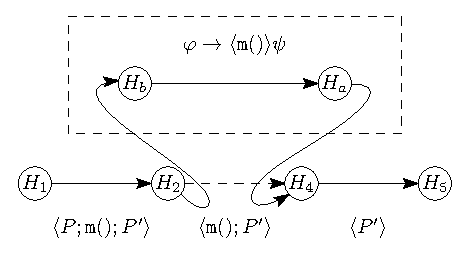
\includegraphics{figures/method_heap.eps}
   \caption{Heaps are `threaded' through method calls. In heap $H_1$ the program fragment $P$ is executed, resulting in heap $H_2$. Either a contract for method \texttt{m()} is employed, which relates the before heap $H_b$ to some heap after the method call $H_a$; or, the method body is unfolded by wrapping it in a method frame that resolves overshadowing of program variables. In both cases, to call the method, heap $H_b$ is equal to $H_2$ and heap $H_a$ is equal to $H_4$. Then the program fragment $P'$ that occurs after the method call is executed using the heap returned by the method.}
   \label{fig:method_heap}
\end{figure}

An important aspect of Java programs are method calls. There are three main issues: calling a method may introduce new program variables that shadow older program variables, calling a method may change the heap, and it is possible to call a method on an object for which its exact type is only known at run-time.

To solve the issue of overshadowing older program variables, KeY uses \emph{method frames}; before a method frame is created, it is ensured that old program variables and new program variables do not collide by renaming the program variables of a method body. Since the \texttt{\textbf{this}} keyword cannot be renamed, the method frame provides a context in which program fragments evaluates \texttt{\textbf{this}} references; it also tracks where the method return value must be placed.

The implicit heap variable is also stored in the method frame, referred to as the before heap. Any heap update within the method is performed on a separate program variable. Statements following a method call are performed using the heap as it is after the method call completes: there are rules for `threading' the heap through a method call, see Figure \ref{fig:method_heap}. There are roughly two ways of treating method calls: unfolding their method body wrapped in a method frame, or using its method contract.

The issue of run-time types is solved using method contracts. Method contracts and other annotations of Java programs are specified in terms of the Java Modeling Language (see~\cite{leavens2013jml}) but with KeY-specific extensions (see \cite[Chapter 7]{KeYbook}). Each method is annotated by a contract that specifies pre- and post-conditions: all implementations of this method should adhere to the contract. The contract determine corresponding correctness formulas in JavaDL: if they are verified, then the corresponding method is correct with respect to its method contract. Consequently, method contracts can be reused in other proofs involving program fragments that call such method.

JML also allows annotations of ghost fields and model fields. Ghost fields are virtual fields that become part of the modelled state of an object on the heap, but are never present when actually executing a Java program. Like normal fields, the value of ghost fields are assigned a default value at object initialization, and can be explicitly changed by JML \texttt{set} annotations. These annotations occur anywhere in method bodies where otherwise a normal statement can be expected. Model fields are introduced as function symbols, and several axioms are added that allow the definition of model fields to be substituted during proof. An example model field is a \emph{class invariant}, which is implicitly assumed to hold of the state of an object between method invocations.

Java programs annotated with JML are entered into the KeY system and the verification begins by generating one or more \emph{proof obligations}. Using the interactive tool, a proof tree is constructed by applying rules until the branches of the tree are closed. Each rule application may result in zero or more branches: in the case of multiple branches, every branch needs to be closed. The tool also provides automation, that automatically applies proof rules using heuristics. This speeds up the verification effort considerably. Finally, after all proof obligations appear as the conclusion of a closed proof tree, the verification effort is done. The proof trees can be stored in a file and reloaded and inspected later.

\section{Class invariant}\label{sec:class-invariant}

We will now formalize a class invariant, thereby characterizing all linked list instances. We focus on unbounded linked lists first, as these are the structures we intend to model. Only at the latest we restrict the size of each linked list to a maximum, as a limitation imposed by the implementation. The setting in which to do our characterization is multi-sorted first-order logic. Our logic is presented in a simplified form, leaving out irrelevant details (such as the heap): the full logic used by KeY is described in Chapter 2 of \cite{KeYbook}.

Consider the following sorts, or type symbols: $\mathit{LinkedList}$ for a linked list, $\mathit{Node}$ for a node, $\mathit{Object}$ for objects and $\mathit{Null}$ for \texttt{null} values. We have a type hierarchy, where $\mathit{Null}$ is related to $\mathit{LinkedList}$ and $\mathit{Node}$, and $\mathit{LinkedList}$ and $\mathit{Node}$ are both related to $\mathit{Object}$. This means that any object of sort $\mathit{Null}$ is also an object of sort $\mathit{LinkedList}$ and $\mathit{Node}$. Moreover, every object that is a linked list is also of type $\mathit{Object}$, and similar for nodes.
We have the following signature: $\mathit{first}: \mathit{LinkedList}\to \mathit{Node}$ and $\mathit{last}: \mathit{LinkedList}\to \mathit{Node}$ for the \texttt{first} and \texttt{last} fields of linked lists, and $\mathit{prev}: \mathit{Node}\to \mathit{Node}$, $\mathit{item}: \mathit{Node}\to \mathit{Object}$, and $\mathit{next}: \mathit{Node}\to \mathit{Node}$ for the \texttt{prev}, \texttt{item} and \texttt{next} fields of nodes. Further, we assume there is exactly one object of $\mathit{Null}$ sort, which is the \texttt{null} constant, for which above functions are left undefined: \texttt{null} is a valid object of the \texttt{LinkedList} and \texttt{Node} Java types, but one may not access its fields.

We search for an axiomatization that characterizes linked lists. One can find these axioms by trial and error. We start listing some obvious axioms:

\begin{enumerate}
    \item $\forall x^\mathit{LinkedList}; (x \neq \mathtt{null} \to (\mathit{first}(x) \neq \mathtt{null} \leftrightarrow \mathit{last}(x) \neq \mathtt{null}))$\\
    Every linked list instance either has both first and last set to \texttt{null}, or both point to some (possibly different) node.
    \item $\forall x^\mathit{LinkedList}; (x \neq \mathtt{null} \to (\mathit{first}(x) \neq \mathtt{null} \to \mathit{prev}(\mathit{first}(x)) = \mathtt{null}))$\\
    The predecessor of the first node of a linked list is set to \texttt{null}.
    \item\label{item:axiom-last} $\forall x^\mathit{LinkedList}; (x \neq \mathtt{null} \to (\mathit{last}(x) \neq \mathtt{null} \to \mathit{next}(\mathit{last}(x)) = \mathtt{null}))$\\
    The successor of the last node of a linked list is set to \texttt{null}.
    \item\label{item:axiom-pred} $\forall x^\mathit{Node}; (x \neq \mathtt{null} \to (\mathit{prev}(x) \neq \mathtt{null} \to \mathit{next}(\mathit{prev}(x)) = x))$\\
    Every node that has a predecessor, must be the successor of that predecessor.
    \item\label{item:axiom-succ} $\forall x^\mathit{Node}; (x \neq \mathtt{null} \to (\mathit{next}(x) \neq \mathtt{null} \to \mathit{prev}(\mathit{next}(x)) = x))$\\
    Every node that has a successor, must be the predecessor of that successor.
\end{enumerate}

These axioms are not yet sufficient: consider a linked list, in which its first and last nodes are different and both have neither a predecessor nor a successor. This linked list should not occur: intuitively, we know that the nodes between first and last are all connected and should form a doubly-linked `chain'. Moreover, for every linked list, this chain is necessarily finite: one can traverse from first to last by following the next reference a finite number of times. This leads to a logical difficulty. Superficially, it is not possible to define the transitive closure of a relation in first-order logic. Let $x$ be a linked list and $y$ a node: we cannot define a formula $R(x,y)$ such that it holds if and only if either $\mathit{first}(x)=y$ or $\mathit{next}^i(\mathit{first}(x))=y$ for some integer $0\leq i$.\footnote{$\mathit{next}^i$ is not a function symbol in first-order logic, but the iteration of $i$ times $\mathit{next}$, where $\mathit{next}^0(x)=x$ and $\mathit{next}^i(x)=next(\mathit{next}^{i-1}(x))$ for all $0<i$.} May there be a different approach to axiomatically characterize linked lists in first-order logic?

\begin{proposition}
It is not possible to axiomatically characterize linked lists with finite chains directly in first-order logic.
\end{proposition}
\begin{proof}
In first-order logic it is not possible to categorically define the natural numbers \cite{benthem2001hol}, meaning there is no set of first-order sentences which has as only model the (standard) natural numbers. Suppose it were definable, then such a set $\Delta$ of first-order sentences exists. Let $n^*$ be the term corresponding to the natural $n$ in the standard model. We may extend the language and include a constant symbol $c$, and let $\Delta^+$ be $\Delta$ together with the sentences $\{0^* < c, 1^* < c, 2^* < c, \ldots\}$. Now take an arbitrary finite subset $\Gamma$ of $\Delta^+$. We know $\Gamma$ has a model: take the standard model and interpret the additional constant $c$ by some \emph{arbitrary} natural number \emph{larger} than every $n$ for which a corresponding term $n^*$ occurs in $\Gamma$. By compactness, $\Delta^+$ has a model too. But since $\Delta^+$ includes $\Delta$, the model for $\Delta^+$ is also a model for $\Delta$. But our model also has an interpretation of $c$: an \emph{infinite} natural number that is larger than all standard natural numbers. This proof is described by Hodges \cite[Chapter 20]{Hodges1983}.

We can consider an embedding from the natural numbers into linked lists. For every natural number $n$, we construct a linked list consisting only of \texttt{null} items with length exactly $n$. The image of this embedding is isomorphic to natural numbers. If linked lists were categorically definable in first-order logic, then the restriction to linked lists consisting only of \texttt{null} items would also be categorically definable. But the latter are isomorphic to natural numbers, that are not categorically definable. Hence, by contraposition, the result.
\end{proof}

The solution is to go beyond first-order logic. We extend our signature to include other sorts: sequences and integers. These sorts have their usual first-order theory. We include a schematic rule to capture integer induction (see \cite[Section 2.4.2]{KeYbook}), which rules out any non-standard model of the integers \cite{benthem2001hol}. Sequences (see \cite[Chapter 5.2]{KeYbook}) have a non-negative integer length $n$, and consist of an element at each position $0\leq i<n$. We write $\sigma[i]$ to mean the $i$th element of sequence $\sigma$, and $\ell(\sigma)$ to mean its length $n$.

Intuitively, each linked list consists of a sequence of nodes between its first and last node. Let $\mathrm{instanceof}_\mathit{Node}: \mathrm{Object}$ be a built-in predicate that states that the object is not \texttt{null} and of sort $\mathit{Node}$. A \emph{chain} is a sequence $\sigma$ such that:

\begin{enumerate}[label=(\alph*)]
    \item\label{item:node} $\forall i^\mathrm{int}; (0\leq i<\ell(\sigma)\to \mathrm{instanceof}_\mathit{Node}(\sigma[i]))$\\
    All its elements are nodes and not \texttt{null}
    \item\label{item:prev} $\forall i^\mathrm{int}; (0<i<\ell(\sigma)\to \mathit{prev}(\sigma[i]) = \sigma[i-1])$\\
    The predecessor of node at position $i$ is the node at position $i-1$
    \item\label{item:next} $\forall i^\mathrm{int}: (0\leq i<\ell(\sigma)-1\to \mathit{next}(\sigma[i]) = \sigma[i+1])$\\
    The successor of node at position $i$ is the node at position $i+1$
\end{enumerate}

Let $\phi(\sigma)$ denote the above property that $\sigma$ is a chain. If $\ell(\sigma)=0$ then $\phi(\sigma)$ is vacuously true: the empty sequence is thus a chain. We now describe properties $\psi_1(\sigma,x)$ and $\psi_2(\sigma,x)$ that relate a chain $\sigma$ to a linked list $x$. These denote the following intuitive properties: there is no first and last node and the chain is empty, or the chain is not empty and the first and last node are the first and last elements of the chain. \begin{equation*}
\begin{split}
\psi_1(\sigma,x) & \equiv (\ell(\sigma) = 0 \land \mathit{first}(x) = \mathit{last}(x) = \mathtt{null}) \\
\psi_2(\sigma,x) & \equiv (\ell(\sigma) > 0 \land \mathit{first}(x) = \sigma[0] \land \mathit{last}(x) = \sigma[\ell(x)-1])
\end{split}
\end{equation*}
\begin{enumerate}\setcounter{enumi}{5}
    \item $\forall x^\mathit{LinkedList}; (x \neq \mathtt{null}\to \exists \sigma^\mathrm{sig}; (\phi(\sigma) \land (\psi_1(\sigma,x)\lor\psi_2(\sigma,x))))$\\
    Every linked list necessitates the existence of a chain of either property
\end{enumerate}

Further, we require that the size field of the linked list and the length of the chain are the same: this property is essential to our verification goal. The size field is modeled by the function $\mathit{size}: \mathit{LinkedList}\to \mathit{int}$, and we require its value (1) to equal the length of the chain, and (2) to be bounded by the maximum value stored in a 32-bit integer. In formulating above properties in JML, we skolemize the existential quantifier using a ghost variable: see Listing~\ref{lst:jml-class-invariant}.

\lstinputlisting[numbers=none,caption={The class invariant of \texttt{LinkedList} expressed in JML.},captionpos=b,label={lst:jml-class-invariant}]{figures/class_invariant.java}

The class invariant is implicitly required to hold for the \texttt{this} object when invoking methods on a linked list instance. In particular, for the constructor of the linked list, the class invariant needs to be established after it returns. In Listing~\ref{lst:jml-constructor}, we state that the constructor always constructs a linked list instance for which its chain is empty. The proof of the correctness follows easily: at construct time, the fields (including the ghost field) of the linked list instance are initialized with their default values. This means the size is zero, and the first and last references are \texttt{null}, and the ghost field is the empty sequence.

\lstinputlisting[numbers=none,caption={The method contract of the constructor of \texttt{LinkedList} expressed in JML.},captionpos=b,label={lst:jml-constructor}]{figures/constructor.java}

For verifying the constructor above, see the video \citeSelf[0:23--0:53]{Bian2020addbranch}, where the relevant video material is between timestamps 0:23 and 0:53.

\section{Acyclicity}\label{sec:acyclicity}

An interesting consequence of the class invariant is the property that \texttt{next} and \texttt{prev} traversal is acyclic. This means that following only \texttt{next} references of any node that is present in a chain never reaches itself, and, similarly for following only \texttt{prev} references.  The acyclicity property implies there is a number of times to follow the \texttt{next} reference until the last node is reached. For the last node, this number is zero (the last node is already reached). The acyclicity property needs to be confused with arbitrary cycles, as there are still cycles present in the linked list structure: for example, in a linked list of size two we can go from one node to the other, by following \texttt{next} and then \texttt{prev}, or the reverse.

We logically specify the acyclicity property as follows. Let $\sigma$ be the chain of a non-empty linked list $x$ for which the class invariant holds. The following holds:
$$
\forall i^\mathrm{int}; (0\leq i<\ell(\sigma)-1\to \forall j^\mathrm{int}; (i < j < \ell(\sigma)\to \sigma[i]\neq\sigma[j]))
$$

\begin{proof}
Let $n$ abbreviate $\ell(\sigma)$. By contradiction: assume there are two indices, $0\leq i<j<n$, such that the nodes $\sigma[i]$ and $\sigma[j]$ are equal.
Then it must hold that for all $k$ such that $j \leq k < n$, the node $\sigma[k]$ is equal to the node $\sigma[k-(j-i)]$:
by induction on $k$.
Base case: if $k = j$, then node $\sigma[j]$ and node $\sigma[j-(j-i)]$ are equal by assumption, since $\sigma[j-(j-i)]=\sigma[i]$.
Induction step: suppose node at $\sigma[k]$ is equal to node at $\sigma[k-(j-i)]$.
We must show if $k+1<n$ then node $\sigma[k+1]$ equals node $\sigma[k+1-(j-i)]$.
This follows from the fact that $\sigma[k+1] = \mathit{next}(\sigma[k])$ and $\sigma[k+1-(j-i)] = \mathit{next}(\sigma[k-(j-i)])$ for $k<n-1$, since $\sigma$ is a chain and the chain property \ref{item:next} of last section.
Now we have established, for all $j \leq k < n$, node $\sigma[k]$ equals node $\sigma[k-(j-i)]$.
In particular, this holds when $k$ is $n-1$, the index of the last node:
so we have $\sigma[n-1] = \sigma[n-1-(j-i)]$.
Since the difference $(j-i)$ is positive, we know $\sigma[n-1-(j-i)]$ is not the last node.
By the linked list property \ref{item:axiom-last} we have $\mathit{next}(\mathit{last}(x))=\mathtt{null}$
and by $\psi_2(\sigma,x)$ we have $\mathit{last}(x)=\sigma[n-1]$:
so we have $\mathit{next}(\sigma[n-1])=\mathtt{null}$.
By the chain properties \ref{item:next} and \ref{item:node} we have $\mathit{next}(\sigma[n-1-(j-i)])=\sigma[n-(j-i)]$
and $\mathrm{instanceof}_\mathit{Node}(\sigma[n-(j-i)])$, respectively.
From the latter we know $\sigma[n-(j-i)]\neq\mathtt{null}$.
So we have $\mathit{next}(\sigma[n-1-(j-1)])\neq\mathtt{null}$.
But this is a contradiction: if nodes $\sigma[n-1]$ and $\sigma[n-1-(j-i)]$ are equal then their \texttt{next} fields must also have equal values, but $\mathit{next}(\sigma[n-1])=\mathtt{null}$ and $\mathit{next}(\sigma[n-1-(j-i)])\neq\mathtt{null}$!
\end{proof}

\lstinputlisting[numbers=none,caption={The method of a lemma added to \texttt{LinkedList} expressed in JML.},captionpos=b,label={lst:jml-lemma}]{figures/lemma_method.java}

For verifying the lemma as formalized in Listing~\ref{lst:jml-lemma}, see the video \citeSelf{Bian2020lemma}.

\section{The \texttt{add} method}\label{sec:add}

Due to the revision of the source code, the add method now calls \texttt{checkSize} first (see Listing~\ref{lst:linkedlist-fix}) to ensure that the size field does not overflow when we add another item. This means that the add method has two expected behaviors: the normal behavior when the length of the linked list is not yet at its maximum, and the exceptional behavior when the length of the linked list is at its maximum.

In the normal case, we expect the \texttt{add} method to add the given argument as an item to the linked list. Thus the sequence of nodes must become larger. We can be specific in the position where we expect the item to be added: to the end of the list. The add method must return true in this case. In the exceptional case, we expect that an exception is thrown. We formalize it in Listing~\ref{lst:jml-add-method}.

\lstinputlisting[numbers=none,caption={The \texttt{add} method with its method contract expressed in JML.},captionpos=b,label={lst:jml-add-method}]{figures/add_method.java}

Since the \texttt{add} method calls the deeper methods \texttt{checkSize} and \texttt{linkLast}, we may employ their method contracts when verifying this method. So, before we verify \texttt{add}, we will first specify and verify these methods.

We expect \texttt{checkSize} to throw an exception if the length of the linked list is too large to add another element, and it returns normally otherwise: see Listing~\ref{lst:jml-check-method} for its specification. Verification of \texttt{checkSize} in both normal and exceptional cases is done automatically by KeY, as can be seen in \citeSelf[0:54--1:24]{Bian2020addbranch}.

\lstinputlisting[numbers=none,caption={The method contract in JML of the \texttt{checkSize} method.},captionpos=b,label={lst:jml-check-method}]{figures/check_method.java}

For the \texttt{linkLast} method, we assume that the length of the linked list is smaller than its maximum length, so we can safely add another node without causing an overflow of the size field. When adding a new node, the resulting chain now is an extension of the previous chain, and additionally the class invariant holds afterwards---this is an implicit post-condition. Since we modify the chain, we need a \texttt{set} annotation that changes the ghost field.

\lstinputlisting[numbers=none,caption={The \texttt{linkLast} method with its method contract expressed in JML.},captionpos=b,label={lst:jml-linklast-method}]{figures/linklast_method.java}

The verification of this method is no longer fully automatic, see \citeSelf[1:25--6:52]{Bian2020addbranch}.

\begin{proof}
Observe that there are two different situations we have to deal with: either the linked list was empty, or it was not. If the linked list was empty, then \texttt{last} is \texttt{null}, and we not only set the \texttt{last} field but also the \texttt{first}. Otherwise, if the linked list was not empty, we update the former last node to set its \texttt{next} field. In the latter case, the challenge is to prove that the class invariant holds after these heap updates. The main insight is that the creation of a new node does not alias with any of the existing nodes, and that the modification of the \texttt{next} field only affects the old last node, see Fig.~\ref{fig:linklast}.

The properties \ref{item:prev}, that fixes \texttt{prev} fields to point to the previous node in the sequence, and \ref{item:next}, that fixes \texttt{next} fields to point to the next node in the sequence, of the chain are the remaning goals in \citeSelf[3:58]{Bian2020addbranch}. Proving \ref{item:prev} is straightforward if one makes a distinction between old nodes and the new node. Proving \ref{item:next} in the `heap after' involves two cases: either the index is between $0$ and less than $\ell(\sigma)-2$, or it used to be the last node and now has index $\ell(\sigma)-2$. In the former case, the heap update has no effect, as we can show that these nodes are separate from the old last node because they differ in the old value of the next field. In the latter case, the heap update can be used to prove the property directly.
\end{proof}

\begin{figure}
   \centering
   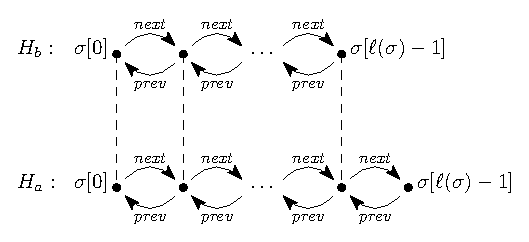
\includegraphics[scale=0.425]{figures/linkedlist-linklast.eps}
   \caption{The heap before ($H_b$) consists of an arbitrary chain of nodes. In the heap after ($H_a$) the dashed lines show which objects are identical to the heap before. The old last node at $\sigma[\ell(\sigma)-1]$ has a different value for its $\mathit{next}$ field in the heap after: this must be the result of a heap update. The new last node does not occur in the heap before: this must be the result of creating a new node.}
   \vspace*{-6pt}
   \label{fig:linklast}
\end{figure}

Finally, we can verify the \texttt{add} method: see \citeSelf[6:58--8:08]{Bian2020addbranch} for the normal behavior case, and \citeSelf[8:09--]{Bian2020addbranch} for the exceptional behavior case.

\section{The \texttt{remove} method}\label{sec:remove}

The \texttt{remove} method takes as argument an object; it searches the linked list for the first node which contains the argument as an item. If found, it unlinks the node from the linked list. Using this intuition, we specify the \texttt{remove} method contract. Like with the \texttt{add} method, there is a deeper method that is called, \texttt{unlink}, which we have to specify and verify first.

An immediate difficulty in specifying the \texttt{remove} method contract is that its intended behavior depends on the behavior of the \texttt{Object.equals} method. Namely, the informal Java documentation states that the first element occurrence in the list that is `equal to' the argument must be removed. Equality can be user-defined by overriding the \texttt{equals} method! We solve this difficulty by assuming a method contract for the equality method, see Listing~\ref{lst:object-equals}.

\lstinputlisting[numbers=none,caption={The \texttt{equals} stub method with its method contract expressed in JML.},captionpos=b,label={lst:object-equals}]{figures/equals_method.java}

We declare the equality method to be strictly pure, which implies that it must be a side-effect free and terminating method (see \cite[Section 7.3.5]{KeYbook}). Each strictly pure method is also directly accessible as an observer symbol (a function symbol) that can be used in specifications (see \cite[Section 8.1.2]{KeYbook}). However, no obvious relation between the possibly overridden equality method and its observer symbol is present. The intention of the contract given in Listing~\ref{lst:object-equals} is to relate the outcome of the method call of \texttt{equals} to the observer symbol $\mathit{equals}$, and this furthermore requires that the implementation is deterministic.

It is not clear what ramifications adding this assumption has. We note that there are Java classes for which equality is not terminating under certain circumstances. Even \texttt{LinkedList} itself does not have a terminating equality, where two linked lists that contain each other may lead to a \texttt{StackOverflowError} when testing their equality. This example is described in the Javadoc \cite{javadoc8collection} of the linked list: ``Some collection operations which perform recursive traversal of the collection may fail with an exception for self-referential instances where the collection directly or indirectly contains itself.'' Another approach is to specify the outcome of equality as referential equality only, e.g. see \cite[Section 4.4]{huisman2002verification}.

Now we can specify the behavior of remove. It can be seen as consisting of two cases: either its result is \texttt{true} and it has removed the first item equal to its argument from the list, or its result is \texttt{false} and the argument was not found and thus not removed. In the first case, the number of elements in the linked list remain unchanged. In the second case, the number of elements decrease by one. See Listing~\ref{lst:remove-method}.

\lstinputlisting[numbers=none,caption={The \texttt{remove} method contract expressed in JML.},captionpos=b,label={lst:remove-method}]{figures/remove_method.java}

It is important to note that we make use of JML's \texttt{\bs old} operator to refer to the equality observer symbol in the old heap. Using equality in the new heap is a different observation; and it should not be possible to verify the remove method in this case. To see why, consider two linked list instances $x$ and $y$: we add $x$ to itself, and to $y$ we add $x$ and then $y$. Now we perform the \texttt{remove} operation on $y$ with $y$ as argument. Clearly $x$ and $y$ are not equal, because they have a different length. But the second item is $y$ itself, and $y$ equals $y$, so it is removed: see Fig.~\ref{fig:remove-equals}. In the resulting heap, both $x$ and $y$ contain $x$ as only item: thus, $x$ and $y$ are equal. If we wrongly observe equality in the new heap, then the implementation would be incorrect: the item to remove should not be the second but the first!

\begin{figure}
   \centering
   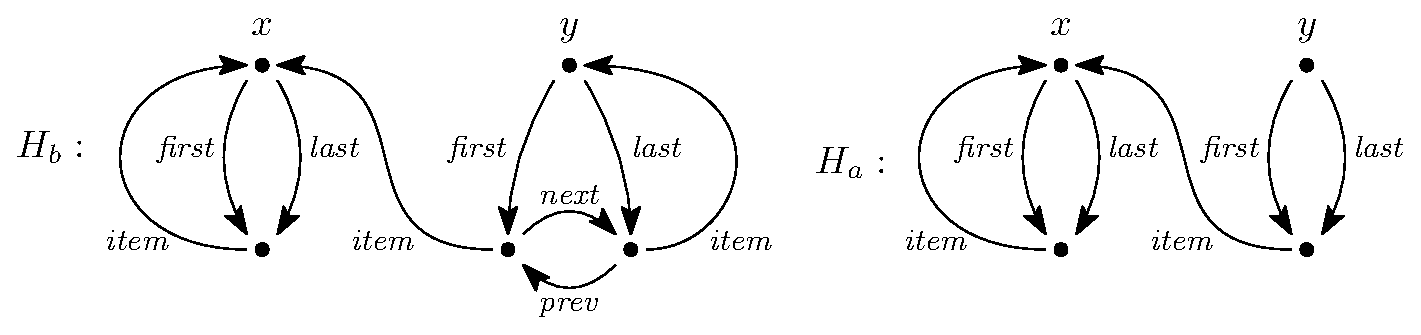
\includegraphics[scale=0.5]{figures/linkedlist-remove-equals.eps}
   \caption{The situation ($H_b$) before \texttt{remove} is invoked on $y$ with argument $y$, and after ($H_a$). The result of this operation is that $y$'s second node is unlinked, hence the first node becomes the last node and its next pointer is cleared: now $x$ and $y$ are equal because they have the same length, and they have the same item, namely $x$.}
   \vspace*{-12pt}
   \label{fig:remove-equals}
\end{figure}

Before we can verify the \texttt{remove} method, we must specify and verify its deeper method: \texttt{unlink}. Within the method of unlink we have to update the chain ghost variable as well, so we add a set annotation to the method body. Additionally, we will make use of the lemma \texttt{lemma\_acyclic} by calling it as a first statement of the method. See Listing~\ref{lst:unlink-method}. This method call is also not present in the original definition for \texttt{unlink}, but we already argued that it does not affect behavior.

\lstinputlisting[numbers=none,caption={The first part of method \texttt{unlink} and its method contract. Note that the @set annotation must not contain a new line, but kept on a single line: otherwise KeY cannot load the source file.},captionpos=b,label={lst:unlink-method}]{figures/unlink_method.java}

An interesting aspect of the specification of \texttt{unlink} is its use of a \emph{ghost parameter}. Although KeY does not directly support ghost parameters, we are able to work around by adding the parameter as a ghost field to our class:
$$\mathrm{//@\ private\ ghost\ \bs bigint\ nodeIndex;}$$
Its value is left undefined for the most part of the lifetime of the linked list, until we are about to invoke \texttt{unlink}. In particular, the ghost parameter contains the index of the node argument, thereby requiring that the node object passed in is part of the chain.



(TODO: unlink verification: four cases, plus intuitive picture, video upload)

(TODO: loop invariants: two cases, video upload)

\section{Conclusion}\label{sec:conclusion}

\begin{exercise}
Change the specifications of the methods to relate the items in the `before heap' to the items in the `after heap'. For example, for the \texttt{add} method, items originally present in the list should still be present at the same place after the method returns. Verify the correctness with respect to this contract.
\end{exercise}

\begin{exercise}
Write a specification and verify the correctness of these linked list methods: \texttt{linkFirst}, \texttt{linkBefore}, \texttt{node}, \texttt{indexOf}, \texttt{clear}.
\end{exercise}

(TODO: exercises)

\bibliographystyleSelf{splncs04}
\bibliographySelf{self}

\bibliographystyle{splncs04}
\bibliography{base}

\end{document}
\endinput
